\documentclass{beamer}

\mode<presentation>
{
  \usetheme{CambridgeUS}      % or try Darmstadt, Madrid, ...
  \usecolortheme{default} % or try albatross, beaver, crane, ...
  \usefonttheme{default}  % or try serif, structurebold, ...
  \setbeamertemplate{navigation symbols}{}
  \setbeamertemplate{caption}[numbered]
} 

\usepackage[english]{babel}
\usepackage[utf8x]{inputenc}
\usepackage{listings}
\usepackage[ampersand]{easylist}



\definecolor{KTI_green}{RGB}{150, 189, 13}
\definecolor{TU_red}{RGB}{255, 55, 81}
\definecolor{faint_gray}{RGB}{180, 180, 180}

\definecolor{syntax_green}{rgb}{0,0.6,0}
\definecolor{syntax_gray}{rgb}{0.9, 0.9, 0.9}
\definecolor{syntax_mauve}{rgb}{0.58,0,0.82}

\lstset{ 
  backgroundcolor=\color{syntax_gray},  % choose the background color
  basicstyle=\scriptsize\ttfamily,        		% size of fonts used for the code
  breaklines=false,                		% automatic line breaking only at whitespace
  captionpos=b,                    		% sets the caption-position to bottom
  commentstyle=\color{syntax_green},    % comment style
  escapeinside={\%*}{*)},          		% if you want to add LaTeX within your code
  keywordstyle=\color{blue},       		% keyword style
  stringstyle=\color{syntax_mauve},     % string literal style
  columns=fullflexible,
  frame=single,
  framesep=0.5cm,
  framexleftmargin=0.5cm,
  xleftmargin=0.5cm,
  framexrightmargin=0.5cm,
  xrightmargin=0.5cm,
  frame=tb,                 
    numbers=left,                    
    numbersep=15pt,  
  }
  
  
\newcommand{\logopython}{\raggedleft 
\includegraphics[height=0.5cm]{logo_python}\hspace{0.1cm}\\\raggedright}
\newcommand{\logopythonbottom}{\raggedleft\vspace{-0.8cm}
\includegraphics[height=0.5cm]{logo_python}\hspace*{0.05cm}\\\raggedright}

\title[BSP05 - Würfelsimulation]{Würfelsimulation}
\author{Dickbauer Y., Moser P., Perner M.}
\institute{PS Computergestützte Modellierung, WS 2016/17}
%\date{Date of Presentation}

\begin{document}

\begin{frame}
  \titlepage
\end{frame}

% Uncomment these lines for an automatically generated outline.
\begin{frame}{Outline}
  \tableofcontents
\end{frame}

\section{Aufgabenstellung}
\begin{frame}{Aufgabenstellung}
Der Benutzer
darf sechsmal eine Zahl raten. Wenn die Zahl größer bzw. kleiner ist als die vom Rechner
gewürfelte Zahl, dann wird dies dem Benutzer jeweils mitgeteilt. Bei richtiger Eingabe
der Zahl gratuliert der Rechner dem Benutzer. Hat der Benutzer mindestens zweimal
richtig oder nie richtig geraten, gibt es spezielle Glückwünsche bzw. Bedauern des Rechners.

\begin{itemize}
  \item Eingabe: geratene Zahl (insgesamt 6x)
  \item Output: Rückmeldung je Durchgang, Endergebnis
\end{itemize}

\end{frame}

\section{Flow Chart}
\begin{frame}{Flow Chart}
	\centering
  	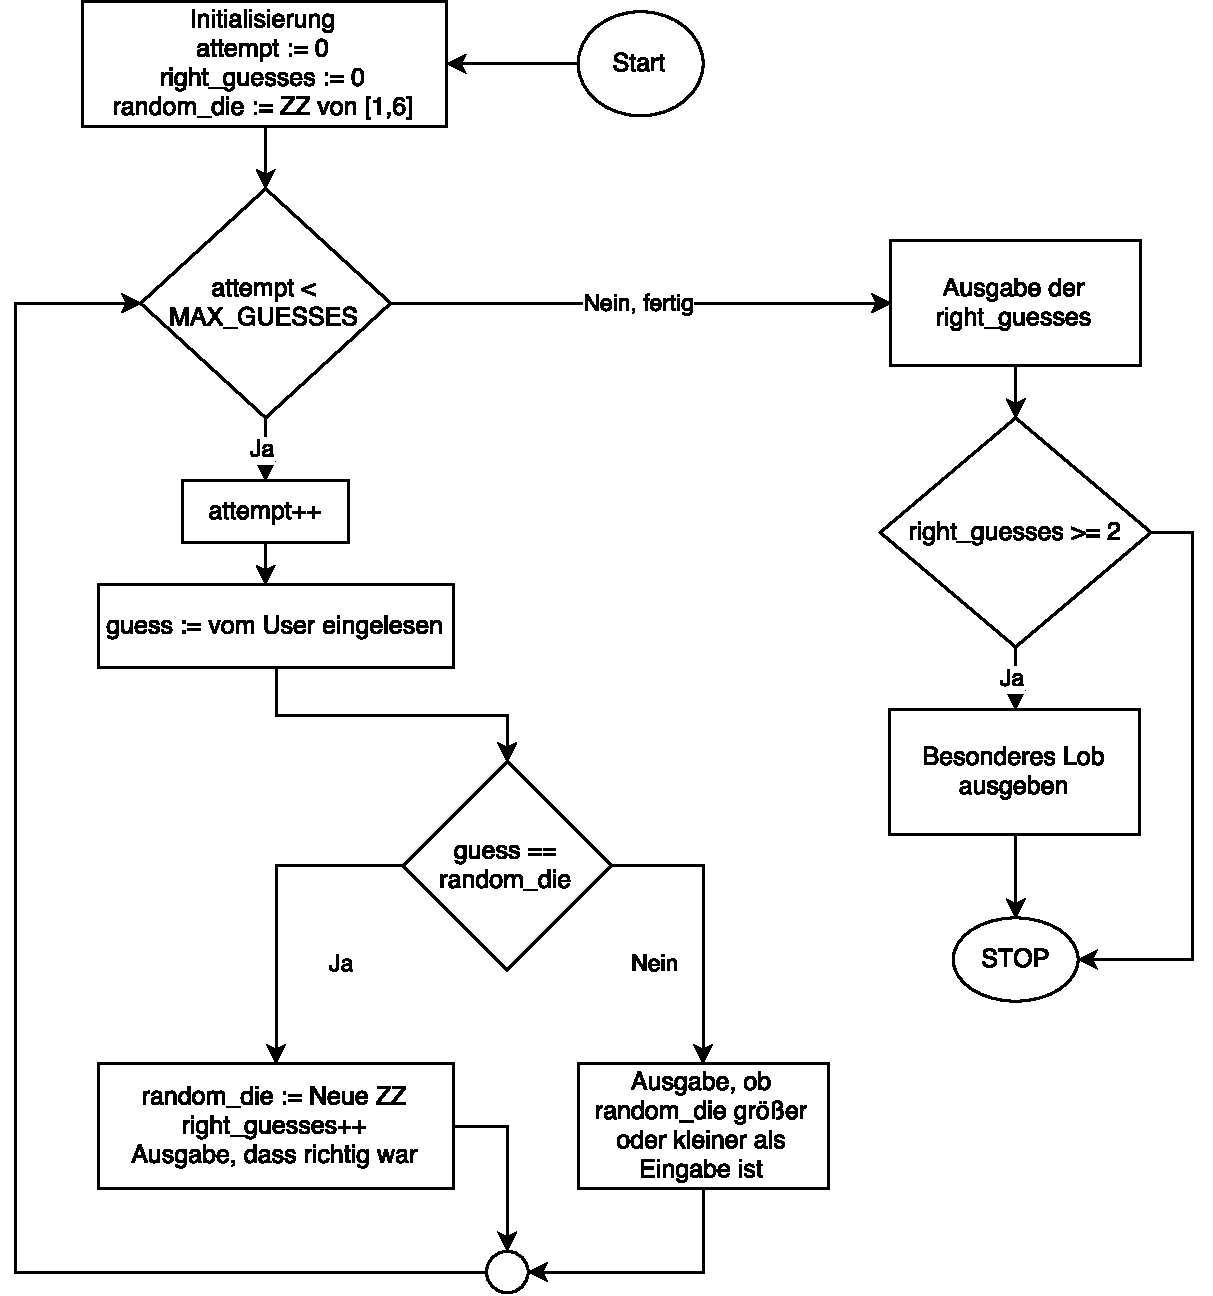
\includegraphics[scale=0.3]{BSP05_Flow_Chart_1.pdf}
\end{frame}
\section{Flow Chart}

\section{Programmcode}
\subsection{Main Funktion}
\begin{frame}[fragile]{Main Funktion - Programmeinstieg}
  \begin{lstlisting}[language=python]
def main():
    attempt = 0
    right_guesses = 0
    random_die = int(random_number_from_interval(0, 6)+1)
    
    while attempt < MAX_NUMBER_OF_GUESSES:
        attempt += 1
        guess = int(input('Rate: '))
        if guess == random_die:
            print('Richtig, du bekommst einen neuen Wuerfel')
            right_guesses += 1
            random_die = int(random_number_from_interval(0, 6)+1)
        else:
            less_or_greater = 'kleiner' if random_die < guess else 'groesser'
            print('Nein, gesuchte Zahl ist {} als {}.'.format(less_or_greater, guess))
    
\end{lstlisting}
\logopythonbottom
\end{frame}

\begin{frame}[fragile]{Main Funktion - Ausgabe der Ergebnisse}
  \begin{lstlisting}[language=python]
    # print result
    print('{} mal richtig geraten'.format(right_guesses))
    if right_guesses == 0:
        print('Kein einziges Mal richtig bei {} Versuchen ist halt kein guter Schnitt...'.format(MAX_NUMBER_OF_GUESSES))
    elif right_guesses >= 2:
        print('Super, mindestens zwei mal richtig, gut gemacht!')
\end{lstlisting}
\logopythonbottom
\end{frame}

\subsection{Verwendete Funktionen}
\begin{frame}[fragile]{Funktion random\_number\_from\_interval(..)}
  \begin{itemize}
    \item Diese Funktion verlangt zwei Eingabeparameter \textit{lower} und \textit{upper}
    \item Gibt eine (pseudo)Zufallszahl (\textit{float}) im Intervall  [\textit{lower}, \textit{upper}) zurück 
    \item \textit{random.random()} ist eine Funktion der Python Standardbibliothek, welche ein Zufallszahl (\textit{float}) im Intervall [\textit{lower}, \textit{upper}) zurück gibt
    \item Mersenne Twister Methode wird als Generator der ZZ verwendet\footnote[frame] {\scriptsize\url{https://docs.python.org/3.5/library/random.html}} \footnote[frame] {\scriptsize\url{https://en.wikipedia.org/wiki/Mersenne_Twister}}
  \end{itemize}
  \begin{lstlisting}[language=python]
def random_number_from_interval(lower, upper):
    val = random.random()
    return lower + (upper -lower) * val
\end{lstlisting}
\logopythonbottom
\end{frame}	
%\begin{frame}[fragile]{Funktion user\_input(input\_vars, [use\_defaults])}
  \begin{itemize}
  	\item Diese Funktion verlang vom User die geforderten Eingabeparameter und gibt diese als von der Programmiererin gewünschten Datentyp wieder zurück
    \item Funktion verlangt als ersten Eingabeparameter die Liste \textit{input\_vars}
    \item Falls \textit{use\_defaults == True} wird der User nicht nach Eingabe gefragt (Dient zum Testen)
    \item Diese Liste besteht wiederrum aus Listen mit je Länge = 3:
    \begin{itemize}
    	\item 0: Text, welcher dem User ausgegeben wird
    	\item 1: Datentyp (int/float/str)
    	\item 2: Default value: Dieser Wert wird zurueckgegeben, falls \textit{use\_defaults == True}
    \end{itemize}
  \end{itemize}
  \begin{lstlisting}[language=python]
x, y = user_input((
    ('Geben Sie einen X Wert ein', int, 10),
    ('Geben Sie einen Y Wert ein', int,  5), False):
  \end{lstlisting}
  \logopythonbottom
\end{frame}	

\section{Beispiel}
\begin{frame}[fragile]{Beispiel anhand fixer Zufallszahlen}
\begin{itemize}
	\item Annahme folgender ZZ und Eingaben:
	\begin{center}
  \begin{tabular}{c|c|c|c|c|c|c}
  \hline 
  Iteration & 0 & 1 & 2 & 3 & 4 & 5\\ 
  \hline 
  ZZ vor iteration    & 3  &  &  & 1  &  & \\ 
  Usereingabe guess  & 1  & 2 & 3 & 4 & 3 & 1 \\ 
  \hline 
  \end{tabular} 
\end{center}
\end{itemize}
\begin{easylist}
\ListProperties(Hide=100, Hang=true, Progressive=3ex, Style*= ,
Style2*=$\bullet$ ,Style3*=$\circ$ ,Style4*=\tiny$\blacksquare$ )
\only<1>{
& Iteration 0:
&& User gibt 1 ein, ZZ ist 3: Programm meldet 'zu niedrig'
&& attempt := 1, right\_guesses := 0
& Iteration 1:
&& User gibt 2 ein, ZZ ist 3: Programm meldet 'zu niedrig'
&& attempt := 2, right\_guesses := 0
& Iteration 2:
&& User gibt 3 ein, ZZ ist 3: Programm meldet 'passt'
&& attempt := 3, right\_guesses := 1
&& Neuberechnung random\_die := 1
}\only<2>{
& Iteration 3:
&& User gibt 4 ein, ZZ ist 1: Programm meldet 'zu hoch'
&& attempt := 4, right\_guesses := 1
& Iteration 4:
&& User gibt 3 ein, ZZ ist 1, Programm meldet 'zu hoch'
&& attempt := 5, right\_guesses := 1
& Iteration 5:
&& User gibt 1 ein, ZZ ist 1, Programm meldet 'passt'
&& attempt := 6, right\_guesses := 2
& While Schleife wird an dieser Stelle beendet, da $attempt \geq 6$
}\only<3>{
\vspace{1cm}
&& Ausgabe, dass 2 richtige sind
&& right\_guesses == 2 $\Longrightarrow$ dem User wird gratuliert 
}
\end{easylist}
\end{frame}

\begin{frame}[fragile]{Anhang: Modifikation des Source Codes um Demo Beispiel zu erhalten}
  \begin{lstlisting}[language=python]
  # Aendere random_number_from_interval() in lib.py wie folgt:
i = -1
ZZ = [3,1] + list(range(1,10))
def random_number_from_interval(lower, upper):
    global i; i += 1;
    return ZZ[i]-1
  \end{lstlisting}
\logopythonbottom
\end{frame}
\end{document}
